\documentclass[12pt]{article}
\usepackage[utf8]{inputenc}
\usepackage[T1]{fontenc}
\usepackage{graphicx}
\usepackage{xcolor}
\usepackage[linewidth=1pt]{mdframed}
\usepackage{xeCJK}
\usepackage{ulem}
\usepackage{color}
%%novalidate

\usepackage{tikz}
\usepackage{calc}
\usepackage{booktabs}


% colors
\definecolor{color1}{HTML}{000060}
%\definecolor{color1}{HTML}{8C260F}
\definecolor{color2}{HTML}{333333}


% fonts
\usepackage{fontspec}
\defaultfontfeatures{Mapping=tex-text}
\setmainfont
[BoldFont=Lato-Bold.ttf,
ItalicFont=Lato-Italic.ttf,
BoldItalicFont=Lato-BoldItalic.ttf]
{Lato-Regular.ttf}
\newfontfamily\headingfont[ItalicFont=Lato-BlackItalic.ttf]{Lato-Black.ttf}
%%%

\usepackage{geometry}
\geometry{a4paper,
hmargin=20mm,vmargin=20mm,
head=0ex,foot=3ex}

\linespread{1.3}

\usepackage[hang]{caption}
\DeclareCaptionFormat{upper}{#1#2\uppercase{#3}\par}
\captionsetup{labelfont={bf,color=color2},textfont={normalsize,color=color2},format = upper,figurename=FIGURE,tablename=TABLE}

%%% fancy sections
\usepackage{titlesec}
%\titleformat{\chapter}{\headingfont\LARGE\bfseries\scshape\color{color1}}{\thechapter}{1em}{}[\titlerule]
\titleformat{\section}{\color{color1}\headingfont\Large\bfseries\uppercase}{\thesection}{1em}{}[\titlerule]
\titleformat{\subsection}{\color{color1}\headingfont\large\bfseries\uppercase}{\thesubsection}{1em}{}
\titleformat{\subsubsection}{\color{color1}\headingfont\bfseries\uppercase}{\thesubsubsection}{1em}{}
%%%

% head and foot
\usepackage{fancyhdr}
\pagestyle{fancy}
\lhead{}
\chead{}
\makeatletter
\rhead{\color{color2}\@date}
\makeatother
\newlength{\myheight}
\lfoot{
\settoheight{\myheight}{\thepage}
\raisebox{-2ex-0.5\myheight}{
\includegraphics[height=4ex]{logo}}
}
\cfoot{\color{color2}\LaTeX\ template for business reports}
\rfoot{\color{color2}\thepage}
\renewcommand\headrulewidth{0pt}
\renewcommand\footrulewidth{0pt}

% custom titlepage
\makeatletter
\newcommand*\DefVar[1]{\@namedef{#1}##1{\global\@namedef{get#1}{##1}}}
\DefVar{summary}
\renewcommand{\maketitle}{
\begin{center}

\begin{tikzpicture}
    \node[draw=none,%color1,line width=0.4pt,
      fill=color1,
      inner sep = 10pt,
      text width=\textwidth-20pt,
      text centered
    ] {\color{white}\headingfont\bfseries\huge\@title};
\end{tikzpicture}

\includegraphics[width=\textwidth]{opening}\par
\headingfont\bfseries\Large\@author\par
\bigskip\medskip
{\color{color2}\normalfont\normalsize\textbf{Summary:}\\
\getsummary}
\end{center}
\clearpage
}
\makeatother
%%%

%%% fancy boxes
\usepackage{tcolorbox}
\usepackage{wrapfig}
\def\fullboxbegin{
\bigskip
\begin{tcolorbox}[colback=color1,colframe=color1,coltext=white,arc=0mm,boxrule=0pt]
}
\def\fullboxend{\end{tcolorbox}\medskip}
%
\def\leftboxbegin{
\begin{wrapfigure}{l}{0.5\textwidth}
\begin{tcolorbox}[colback=color1,colframe=color1,coltext=white,arc=0mm,boxrule=0pt]
}
\def\leftboxend{
\end{tcolorbox}
\end{wrapfigure}
}
%
\def\rightboxbegin{
\begin{wrapfigure}{r}{0.5\textwidth}
\begin{tcolorbox}[colback=color1,colframe=color1,coltext=white,arc=0mm,boxrule=0pt]
}
\def\rightboxend{
\end{tcolorbox}
\end{wrapfigure}
}
%
\newcounter{frames}
\def\frameboxbegin#1{
\bigskip
\refstepcounter{frames}
\begin{tcolorbox}[colback=white,colframe=color1,arc=0mm,title={\MakeUppercase{\textbf{Frame \arabic{frames}}: #1}}]
}
\def\frameboxend{
\end{tcolorbox}
}
%%%

\usepackage{lipsum}


\usepackage{tikz,mathpazo}
\usetikzlibrary{shapes.geometric, arrows}
\usetikzlibrary{calc}


\title{Digital Clock - JEHHEJ}
\author{JEHHEJ\\ Huangyq /Hongry }
\date{\today}
\summary{ A LED digital clock
}


\begin{document}
\maketitle

\tableofcontents
\clearpage

\section{Introduction}
	The basic task of the project of LED
Digital Clock is to use DC power to 
finally make a clock. And we add two
additional functions—alarm and day 
display—into our circuit. The highlight 
among all these functions is that we use
logic gate to build a unique encoder 
ourself for 7 LED indicating days form 
Monday to Sunday.
\section{Flow Chart}
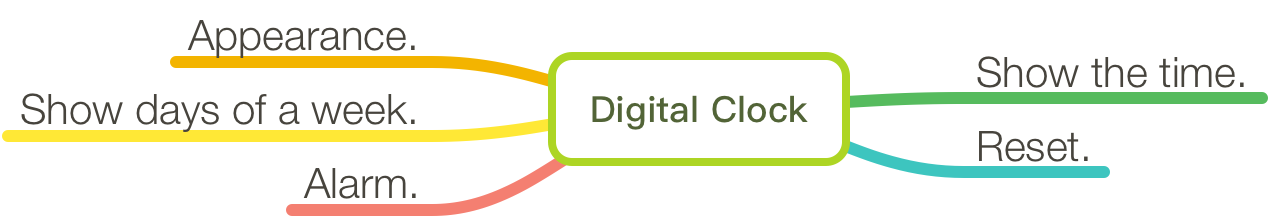
\includegraphics[scale=0.75]{workflow}


\section{Circuit Principle}
What we have learnt from Electric 
Circuits Lab is the usage of 555 Timer 
and some simple logic calculation. 
However, we are not familiar with Flip-
Flop and Seven Segment Display and its 
encoder—74LS48. Through the help of our 
TA especially his sending a material of 
the principle of Flip-Flop and some 
materials on the Internet, we simulate 
and build our circuit successfully. Here 
are some principle of the basic 
components applied into our circuit.
\subsection{JK Flip-Flop}
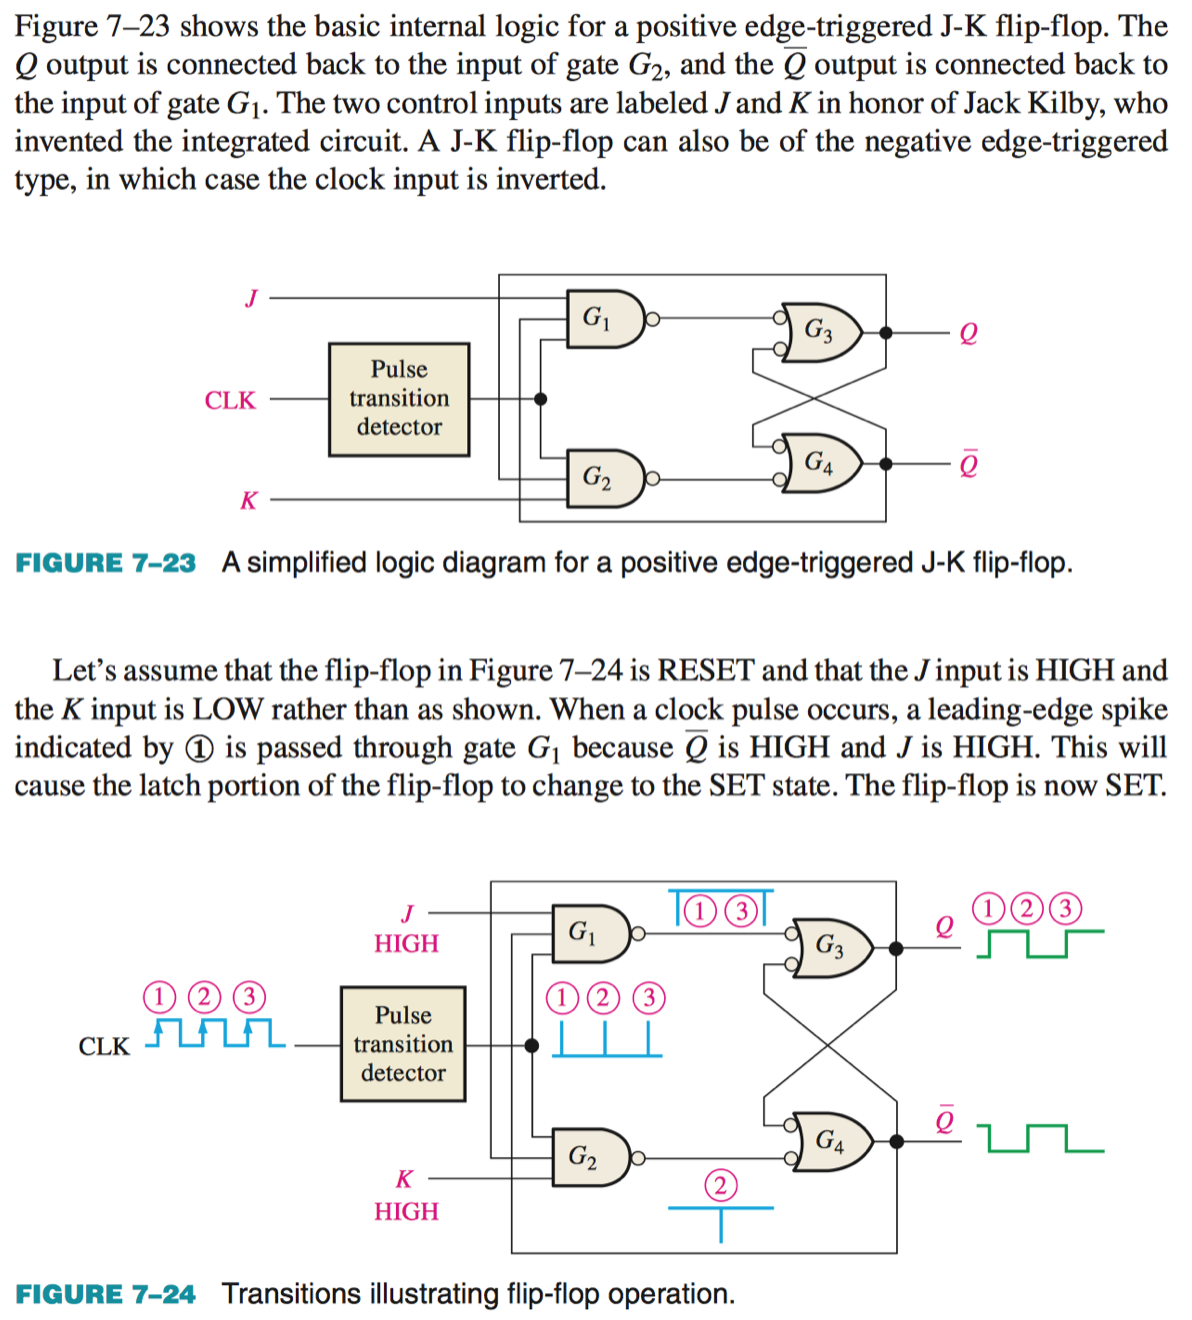
\includegraphics[scale=0.7]{JK.png}\\
Source: Digital Fundamental Chapter 
Flip-Flops

\subsection{555 Timer}
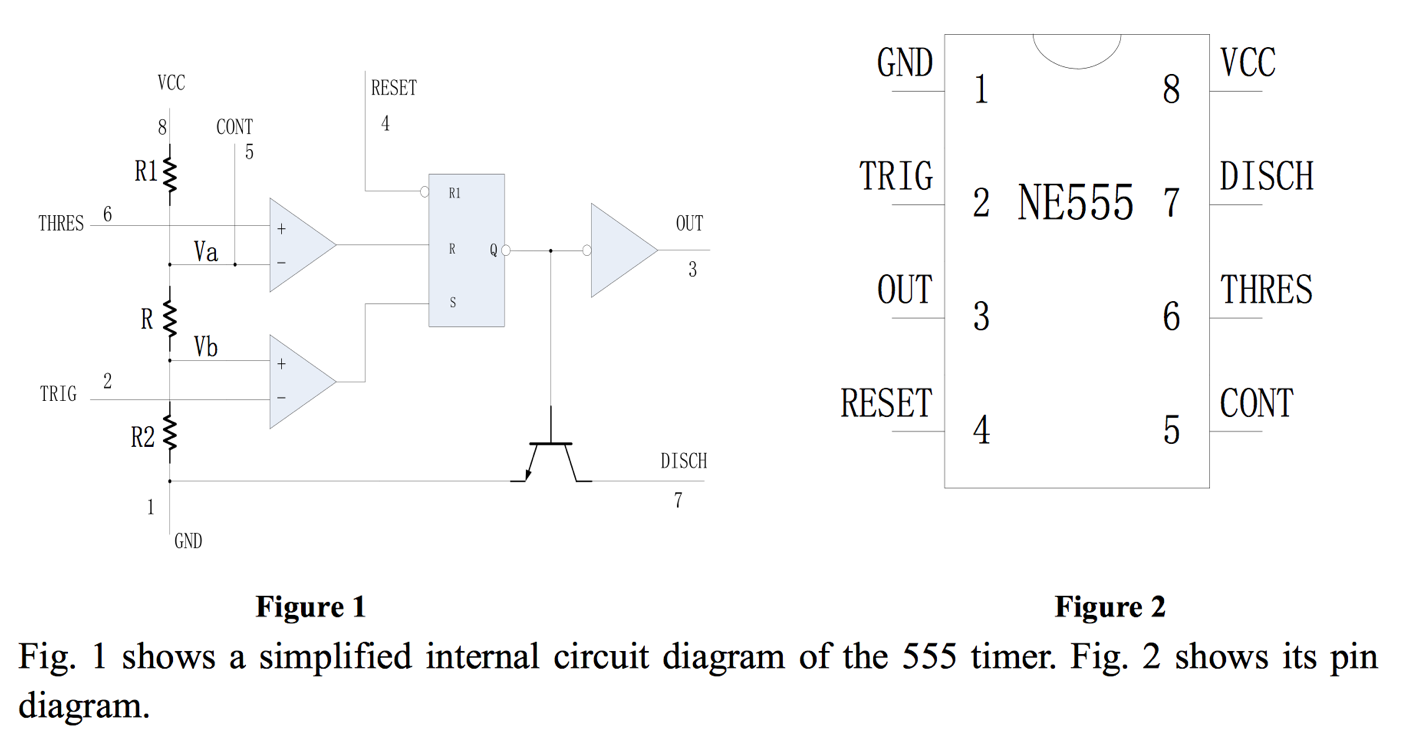
\includegraphics[scale=0.7]{555.png}\\
Source: UC Berkeley, EECS100 Lab, Fall 
2009.

\subsection{PMOS}
When the voltage of input A is high, the PMOS transistor is in an OFF (high resistance) state so it would limit the current flowing from the positive supply to the output, while the NMOS transistor is in an ON (low resistance) state, allowing the output from drain to ground. Because the resistance between Q and ground is low, the voltage drop due to a current drawn into Q placing Q above ground is small. This low drop results in the output registering a low voltage.\\
Source: https://en.wikipedia.org/wiki/CMOS\\
\clearpage

\section{Components}
\begin{table}[!h]
\centering
\caption{Component List.}
\begin{tabular}{ccc}
\toprule
Name & Type  & Quantity \\
\midrule
 Battery Box  &    & 1  \\
 Timer555 &   & 1 \\
 Capactior  & 0.01$\mu$F   & 1  \\
     & 0.1$\mu$F  & 1 \\
Resistor & 1k$\Omega$  & 1 \\
     &  2k$\Omega$ & 1 \\
     &  100$\Omega$ & 3 \\
JK Flip Flop   & 74HC112  & 27 \\
Seven Seg Display  &    & 12  \\
Seven Seg Encoder&  74LS48D  & 12  \\
Switch  &    & 10  \\
NOT Gate  & 74AS04M & 20  \\
NAND Gate  & 7400N & 20  \\
XOR Gate  & 7486N & 10  \\
OR Gate  & 7432N & 5  \\
Piezo Buzzer & & 1  \\
CMOS & IRF510 & 4  \\
LED & White & 10  \\
\bottomrule
\end{tabular}
\end{table}

\clearpage


\section{Block Schematic}

\thispagestyle{empty}
\tikzstyle{startstop} = [rectangle, rounded corners, minimum width=3cm, minimum height=1cm,text centered, draw=black, fill=red!30]
\tikzstyle{io} = [trapezium, trapezium left angle=70, trapezium right angle=110, minimum width=1cm, minimum height=0.8cm, text centered, draw=black, fill=orange!30]
\tikzstyle{process1} = [rectangle, minimum width=3cm, minimum height=1cm, text centered, text width=3cm, draw=black, fill=yellow!30]
\tikzstyle{process2} = [rectangle, minimum width=3cm, minimum height=1cm, text centered, text width=3cm, draw=black, fill=blue!30]
\tikzstyle{process3} = [rectangle, minimum width=3cm, minimum height=1cm, text centered, text width=3cm, draw=black, fill=brown!30]
\tikzstyle{process4} = [rectangle, minimum width=3cm, minimum height=1cm, text centered, text width=3cm, draw=black, fill=green!30]
\tikzstyle{decision} = [diamond, minimum width=3cm, minimum height=1cm, text centered, draw=black, fill=green!30]
\tikzstyle{arrow} = [thick,->,>=stealth]

\begin{tikzpicture}[node distance=2cm]
\node (start) [startstop] {Power Supply 6V};
\node (in) [startstop, above of=start, yshift=0.5cm, xshift=2cm, yshift=1cm] {Function generator};
\node (pro1_1) [process1, right of=start, xshift=2cm] {Turn On/Off Time Ajustment Part};
\node (pro1_2) [process1, right of=pro1_1, xshift=2cm] {Reset Ajustment};
\node (pro2_1) [process2, above of=pro1_1, yshift=0.5cm,xshift=2cm] {Counter};
\node (pro2_2) [process2, above of=pro2_1] {Encoder};
\node (pro2_3) [process2, above of=pro2_2] {Seven Seg Display};
\node (pro3_1) [process3, right of=pro2_1, xshift=2cm] {DIY Encoder};
\node (pro3_2) [process3, right of=pro3_1, xshift=2cm] {7 LEDs\\(to represent for days from Mon. to Sun.)};
\node (pro4_1) [process4, below of=pro1_1, yshift=-0.7cm] {Set OR Part};
\node (pro4_2) [process4, right of=pro4_1, xshift=2cm] {Comparison Part};
\node (pro4_3) [process4, below of=pro4_1] {Turn On\&Off Alarm Part};
\node (pro4_4) [process4, right of=pro4_3, xshift=2cm] {Setting Part Via Counter};
\node (pro4_5) [process4, below of=pro4_4] {Encoder};
\node (pro4_6) [process4, below of=pro4_5] {7 Seg Display};
\node (pro4_7) [process4, right of=pro4_2, xshift=2cm] {7 Seg Display};

\draw [arrow](start) -- (pro1_1);
\draw [arrow](start) |- (pro2_1);
\draw [arrow](start) |- (pro2_2);
\draw [arrow](start) -- (0,1.5) -| (pro3_1);
\draw [arrow](start) -- (0,-5.9)-- (7,-5.9)--(7,-5.3);
\draw [arrow](start) -- (0,-1.5) -| (pro4_2);
\draw [arrow](pro2_1) -- (6,-2.7);
\draw [arrow](pro1_2) -- (pro2_1);
\draw [arrow](in) -- (pro2_1);
\draw [arrow](pro2_1) -- (pro3_1);
\draw [arrow](pro3_1) -- (pro3_2);
\draw [arrow](pro1_1) -- (pro1_2);
\draw [arrow](pro2_1) -- (pro2_2);
\draw [arrow](pro2_2) -- (pro2_3);
\draw [arrow](start) |- (pro4_1);
\draw [arrow](start) |- (pro4_5);
\draw [arrow](pro1_1) -- (pro1_2);
\draw [arrow](pro1_1) -- (in);
\draw [arrow](pro4_1) -- (pro4_2);
\draw [arrow](pro4_2) -- (pro4_7);
\draw [arrow](pro4_3) -- (pro4_1);
\draw [arrow](pro4_3) -- (pro4_4);
\draw [arrow](pro4_4) -- (pro4_5);
\draw [arrow](pro4_5) -- (pro4_6);

\end{tikzpicture}
\frameboxbegin{Color Block}
Red Block: Input\\
Purple Block: Basic Digital Clock\\
Yellow Block: Time Adjust Part\\
Brown Block: Show-Day Part\\
Green Block: Alarm Part
\frameboxend
\clearpage

\subsection{Input}
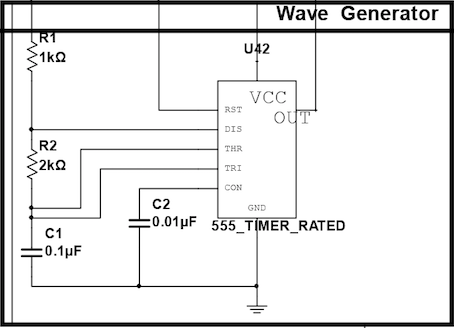
\includegraphics{Input.png}

\subsection{Basic Digital Clock}
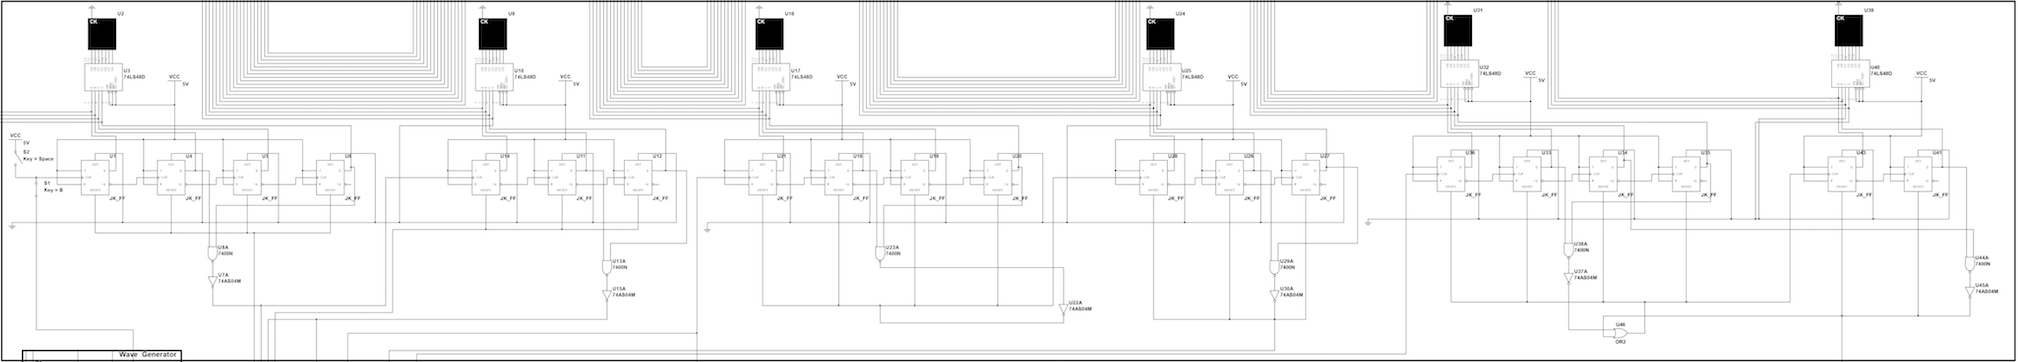
\includegraphics[scale=0.53]{Basic.png}


\subsection{Time Adjust Part}
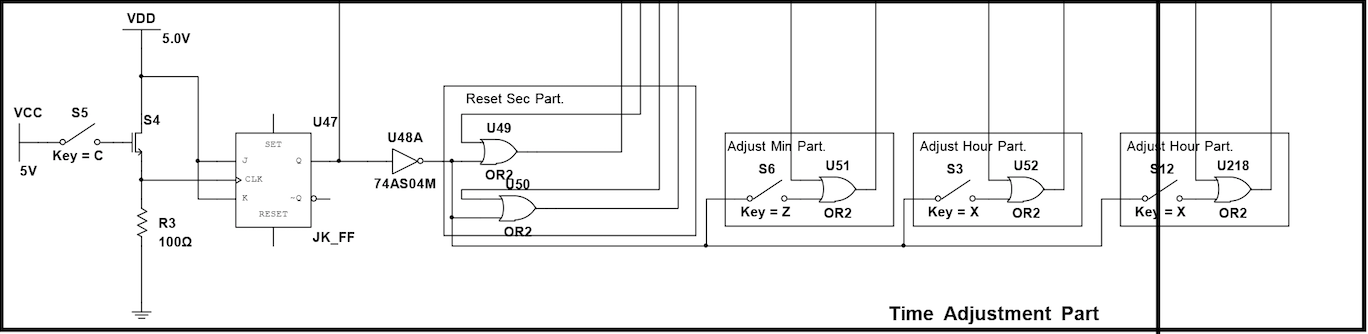
\includegraphics[scale=0.70]{Time.png}

\subsection{Show-Day Part}
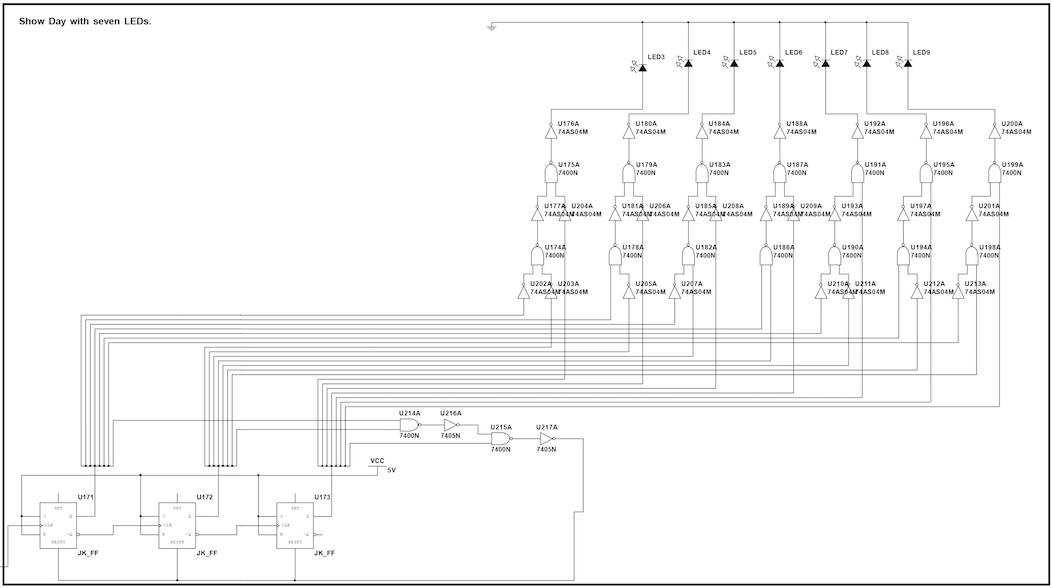
\includegraphics[scale=0.90]{Day.png}
\frameboxbegin{Tips}
Using 7 Led Lights to indicate From Mon. to Sun.
\frameboxend

\subsection{Alarm Part}
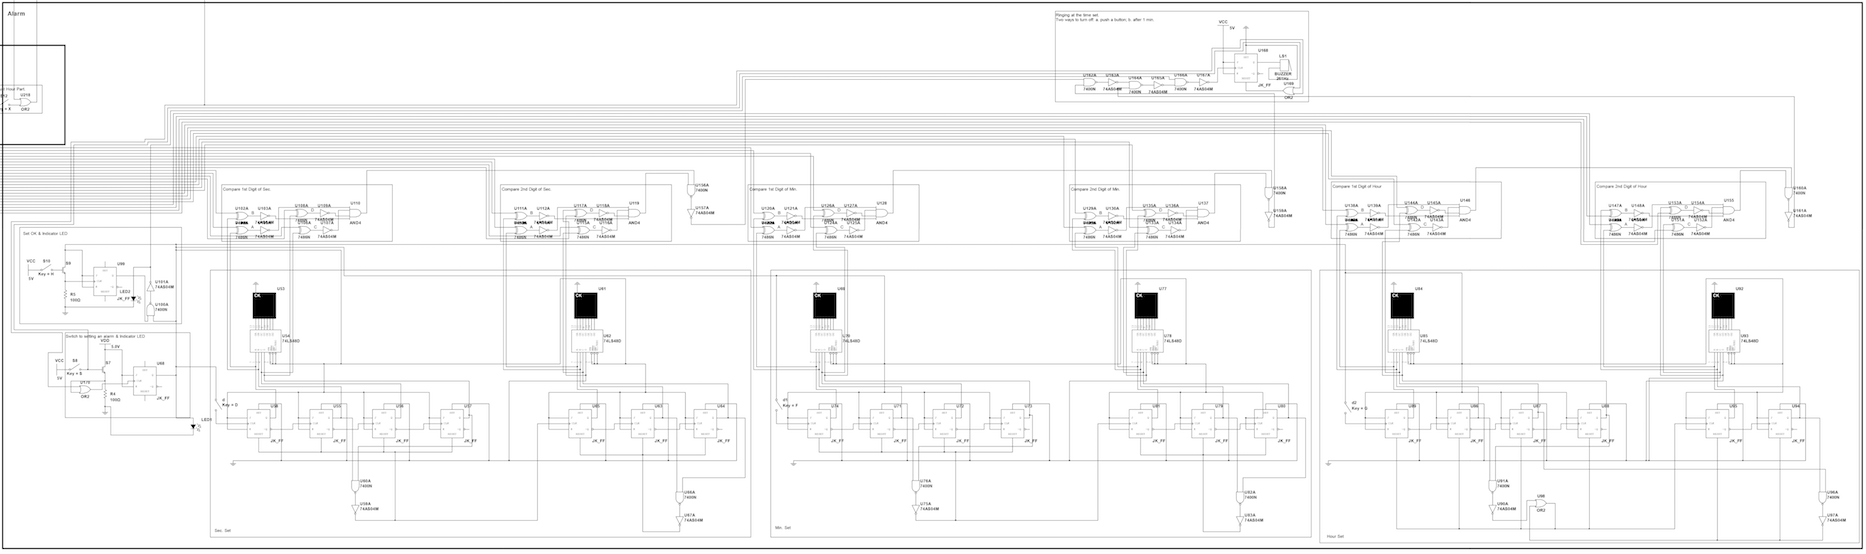
\includegraphics[scale=0.55]{Alarm.png}

\clearpage

\section{Schematic Diagram}
\includegraphics[scale=0.18]{Simulation.png}\\

\section{Achievement}   
Lapping circuit was not so successful to be honest. We have achieved most of our functions last Saturday, but because we bound the maximum current inappropriately, the first model was destroyed. \\
\begin{center}
\fbox{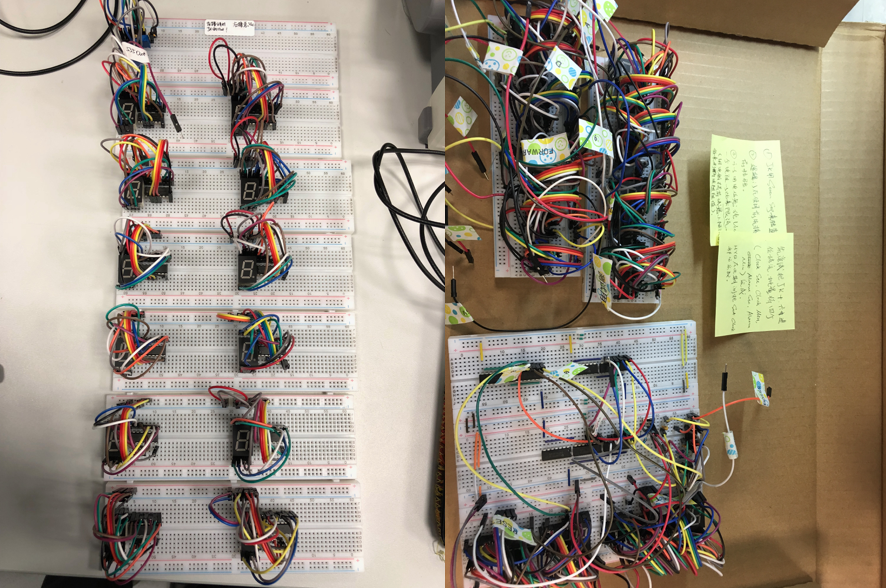
\includegraphics[scale=1]{Achievement.png}}
\end{center}
It taught us a lesson that making the circuit readable and using some indicator to suggest us when something goes wrong immediately. \\
Here is our final achievements.\\
\begin{center}
\fbox{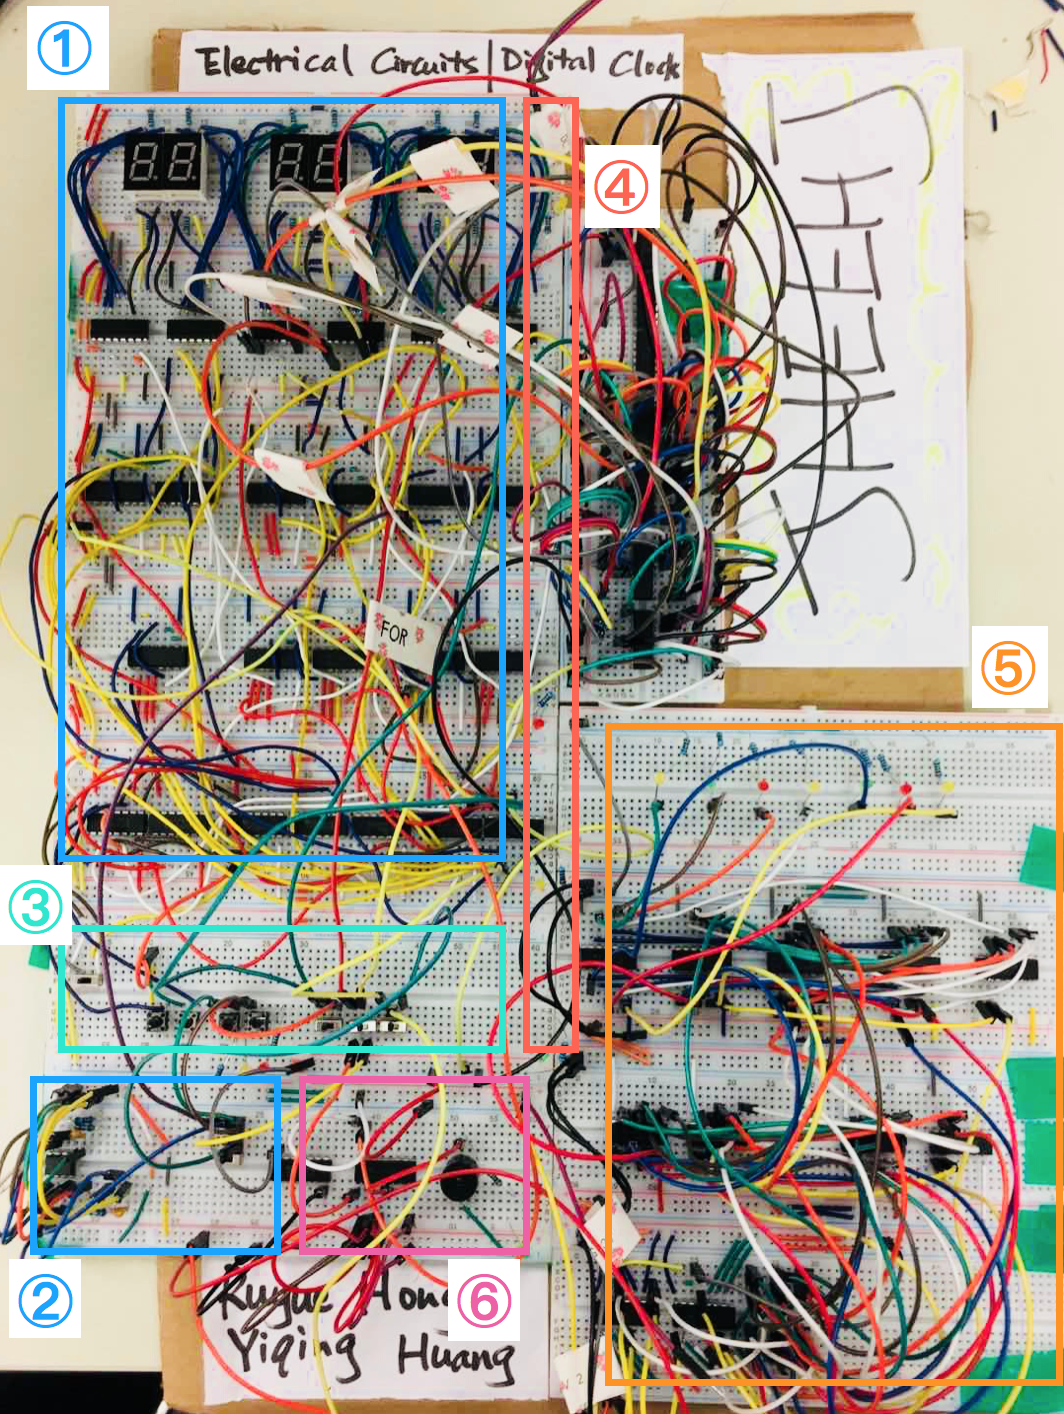
\includegraphics[scale=0.85]{Final.png}}
\end{center}
\clearpage

\begin{enumerate}
	\item Clock: We use Flip-Flop (74LS112) to count square waves generated from 555 Timer. And some logic gates (NAND—74LS00, NOT—74LS04, OR—74LS32) are applied to carry bit. Seven-Segment Display and its matched encoder (74LS48) are the indicator to show the time (the result).
	\item Square Wave: We use 555 timer and some resistors and capacitors to generate square waves.
	\item Time Adjustment Part: When turning on the set button, \uline{the two numbers which show the second of the clock will be reset to zero} . At the beginning, we supposed to use PMOS to generate square waves on our own to adjust time, but failed. So we changed our mind and \uline {use the square waves generated from 555 timer part to adjust minute, hour and day part of the clock}.
	\item Error Indicators: We \uline{set a LED on every bread board} and they will show us which part goes wrong as soon as an error occurred \uline{by turning off or twinkling}. It looks very simple, but it is actually convenient and efficient. It do have helped us find a destroyed Flip-flop and several careless mistakes in connecting circuits.
	\item Days Indicator: We use 7 LEDs from left to right to represent for Monday to Sunday. To achieve this goal, unlike a Seven-Segment Display which has a matched encoder, \uline{we use logic gates which cost 3 bread boards to build an encoder on our own}. Of course, Flip-Flops are used to count the number.
	\item Hour Alarm: When time goes from an hour to another, the beeper \uline{will beep for 10 seconds as we designed}. We use a Flip-Flop to receive a signal from hour carry bit, so when it comes to an new hour, the Q of the Flip-Flop will turn from LOW to HIGH and the beeper will keep beeping. Besides, the reset port is connected to the 10-second carry bit so that when 10 seconds after now time, Q will turn from HIGH to LOW, so the beeper will stop to beep.
\end{enumerate}

\section{Presentation and Poster}
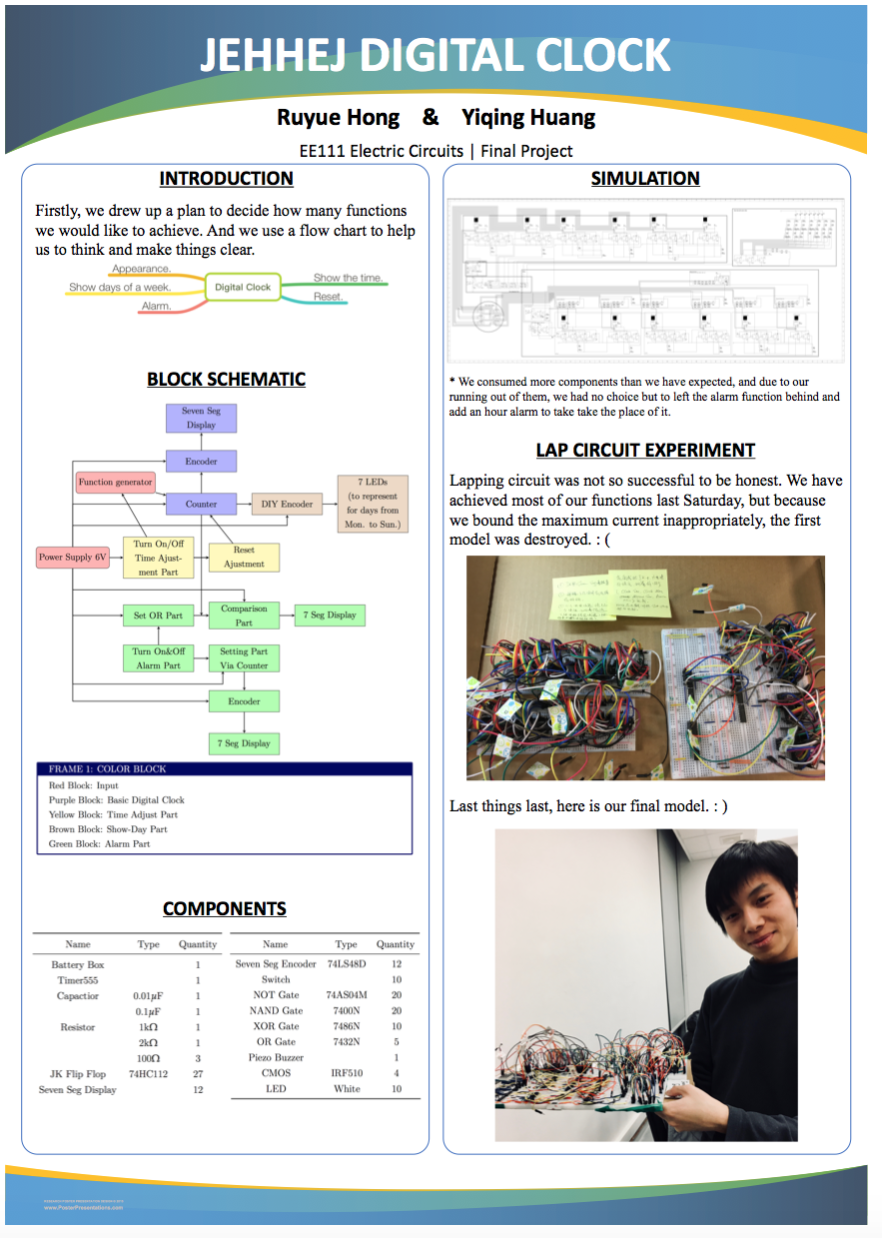
\includegraphics[scale=1]{poster.png}


\section{Little Thoughts}
\par\setlength{\parindent}{2em}
We picked up this project because we truly love it. So we made efforts to it and run out of our comfort zone. We struggle till the last minute to finish as more functions as we can.
To be honest, it is a pity that we lack time to reach our original goal to build a alarm. However, I am so glad that we can find a plan B and bring it into the actual circuit in a short time. 
Ruyue is my best partner. We work out our plan smoothly and we exchange our ideas as soon as they came out of our minds. We sometimes argued with each other for our own thoughts or solutions to solve a specific problem and it do result in our remarkably high efficiency. We know when to stop and have a short break and when to insist on. We inspired each other when we were gotten in a dilemma and then fight a way out. 
Maybe I will never make a second digital in the future but the experience in how to design a circuit, how to learn the usage of components in a fast way and most crucially how to fix unknown bugs in circuits must be rooted in my mind. And this is the essence of this course regardless of the result and the grade, which is extremely helpful. 
Last but not least, thanks for my TA Shuo Ni, and thanks for my best partner Ruyue.\\
—— Yiqing Huang\\


Looking back on the week that past by, everyday is filled with depression and sudden surprise. Before entering the lab first time, we are occupied with fancy imagination that except accomplishing the required electric circuit we can even build an awesome appearance to cover the circuit which makes it like a real clock in our daily life, thus replacing the old clock with the home-made one. This kind of imagination continued even after the period we build the circuit first time. However, too many seemingly unsolvable bugs destroy our dream. It is easy for us to transfer the simulating one to real electric circuit, however, everyday we spend a large amount of time to figure out the reason why it fails to function even if the Multism runs successfully. I picked up the project simply out of my adoration. We came to the lab everyday with full enthusiasm, but it damped my passion gradually over time. \\
	Those days are like the dark sky I saw every time I walked back to the dormitory with my partner. The little shining stars scattering above are like the final presentation which are shown to others. The darkness around the stars are just our normal days spent in the lab. Our depression , hundreds of time willing to give up combined with little success and sudden surprise are deeply hidden in the darkness which are only shown to us own. \\
	Fortunately, our effort are not in vain, we work things out in the end. During the process to the final point, we are so worried about whether our time and effort will just be a speck of dusk in the galaxy or become the stars lighting up our days. But now, I have to admit that it is not the stars but the darkness that actually form the sky. We have to be thankful to ourselves, it is us who choose to keep on walking even our enthusiasm fading over time. We have to be thankful to my dear partner, who choose to accompany me walking under the dark sky even if he is so tired, even if I am so impatient with him. The final design is different from the initial one. It combined with the fancy ideas of Xiaoqingqing and me, it is also the outcome of our hundreds time of argument. .. so many words are just on the tip of my tongue but hard to speak them out. Never mind, just let them hidden in the dark sky as well, hidden in the days we passed by, buried in our own memory.\\
	—— Ruyue Hong\\

\section{Reference}
\begin{itemize}
\item Digital Fundamental Chapter 7 Flip-Flops.
\item UC Berkeley, EECS100 Lab, Fall 2009.
\item https://en.wikipedia.org/wiki/CMOS.
\end{itemize}
\end{document}



